\documentclass[11pt]{article}

% ------------------------------------------------------------- packages
\usepackage[margin=1in]{geometry}
\usepackage{amsmath, amssymb}
\usepackage{graphicx}
\usepackage{booktabs}
\usepackage{array}
\usepackage{float}
\usepackage{caption}
\usepackage{subcaption}
\usepackage{hyperref}
\usepackage{xcolor}
\hypersetup{colorlinks=true, linkcolor=blue!50!black,
            citecolor=blue!50!black, urlcolor=blue!50!black}
\usepackage{enumitem}
\setlist{itemsep=2pt, topsep=2pt}

\graphicspath{{figures/}}

\title{Capital Bikeshare Hourly Demand:\\
       Clustering, Factor Analysis, and Lasso}
\author{Glen Morgenstern, Lienne Childs, Jonathan Kim, Ziang Yuan}
\date{STAT32950 Spring 2026}

\begin{document}
\maketitle

\section{Introduction}

\paragraph{Dataset.}
The Capital Bikeshare hourly demand dataset records every hour of operation of the Washington D.C.\ bikeshare
system from 2011-01-01 to 2012-12-31, together with calendar and weather covariates. It contains $n=17{,}379$ rows and 18 columns with no missing values. Our target variable is \texttt{cnt}, the total number of rentals during the hour.

\paragraph{Research question.}
We derived the following question from some exploration and obervation on the dataset, which we will introduce later. What variables might drive hourly bike-rental demand in Washington D.C., and how can we predict cnt more precisely with these variables?
We attack this question with three complementary methods:
\begin{enumerate}
\item \textbf{Clustering} (K-means), with \texttt{cnt} included in the
      feature set, to discover demand regimes.
\item \textbf{Factor analysis} (three factors, varimax rotation) on
      the same numeric block plus \texttt{yr}, to identify the
      latent factors organizing the joint variation and how
      \texttt{cnt} loads onto them.
\item \textbf{Lasso regression} of $\log(1+\texttt{cnt})$ on all
      other variables, read as a path across $\lambda$ rather than as a single ``best'' model: we report 5-fold CV-based choices and also examine more aggressive $\lambda$ values to see which variables Lasso retains under stronger sparsity.
\end{enumerate}
We then compare what each method answers, what it reveals, and how
the conclusions differ.

\paragraph{Preprocessing.}
We drop \texttt{atemp} (collinear with \texttt{temp}, $r=0.99$); we
merge \texttt{weathersit}=4 (only $3$ rows) into \texttt{weathersit}=3
for the supervised models; we standardize all numeric inputs to
mean $0$, variance $1$ before clustering, factor analysis, and
Lasso so that magnitudes are comparable. We do not use
\texttt{casual} or \texttt{registered} as predictors because they
sum identically to \texttt{cnt}.

% =====================================================================
\section{Exploratory data analysis}

We begin with a brief, methodologically simple but
variable-complete description of the target and its pairwise
relationship with every other variable in the dataset
(Figures~\ref{fig:cnt-dist}--\ref{fig:corr}).

\begin{figure}[H]
\centering
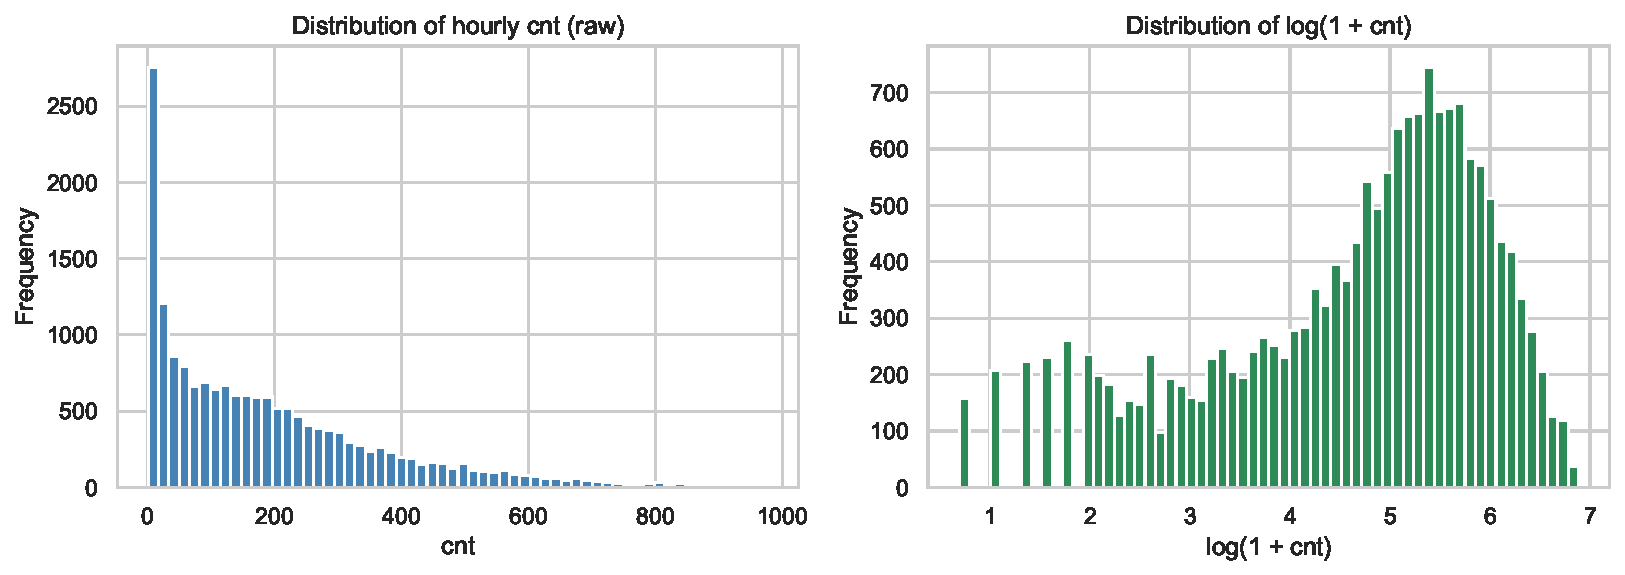
\includegraphics[width=0.95\linewidth]{fig01_cnt_distribution.pdf}
\caption{Distribution of hourly \texttt{cnt}: raw (left) and after
$\log(1+\cdot)$ (right). The raw target is heavily right-skewed
(skewness $\approx 1.28$); the log transform brings the skewness to
$\approx -0.82$ but reveals a clear bimodality, an early hint
of two latent demand regimes.}\label{fig:cnt-dist}
\end{figure}

\begin{figure}[H]
\centering
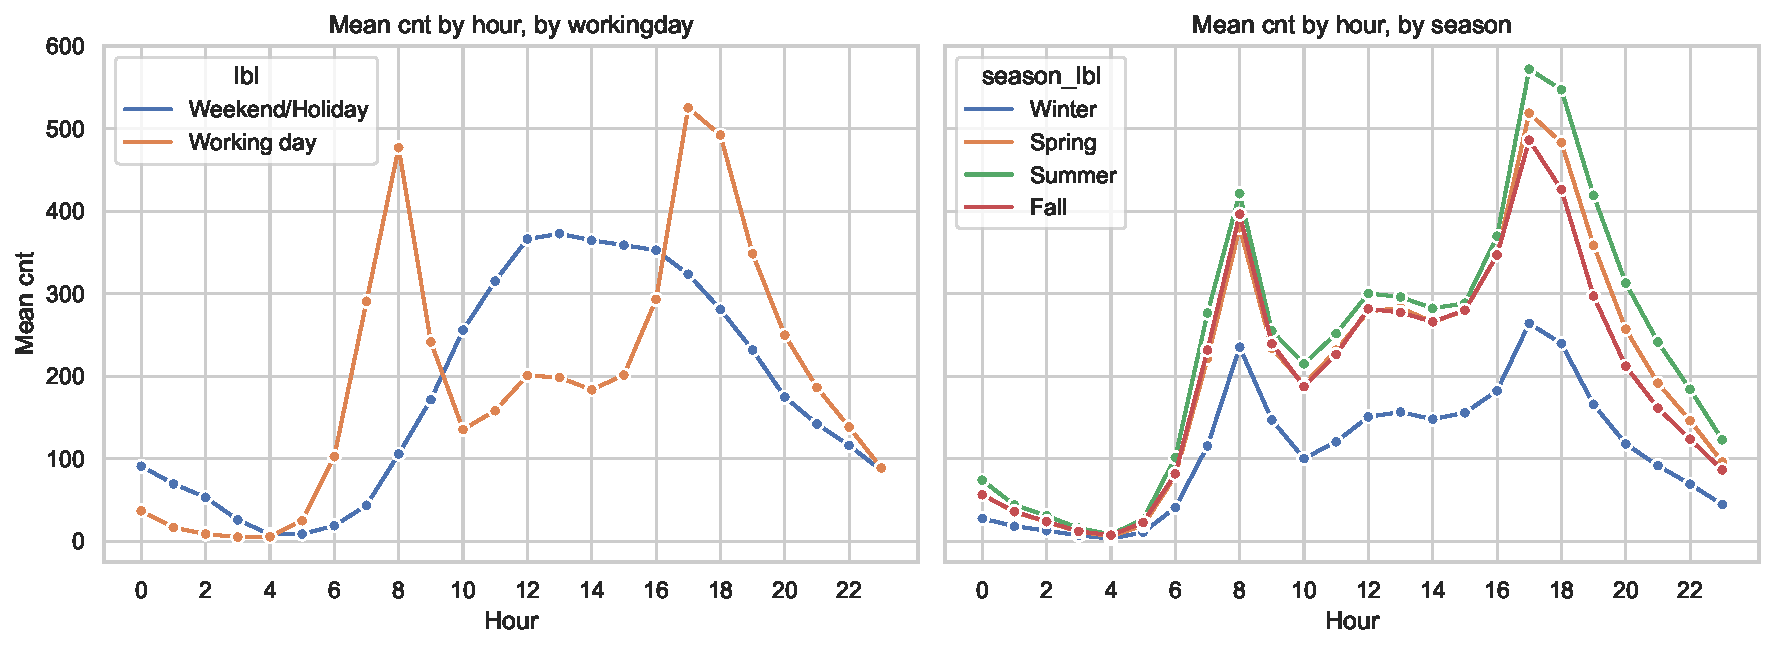
\includegraphics[width=0.95\linewidth]{fig02_hourly_patterns.pdf}
\caption{Mean \texttt{cnt} by hour-of-day. Left: split by
\texttt{workingday}; the sharp bimodal commuter signature at
08:00 and 17:00--18:00 is the most distinctive feature of the
dataset. Right: by season; season scales the curve but does not
reshape it.}\label{fig:hourly}
\end{figure}

\begin{figure}[H]
\centering
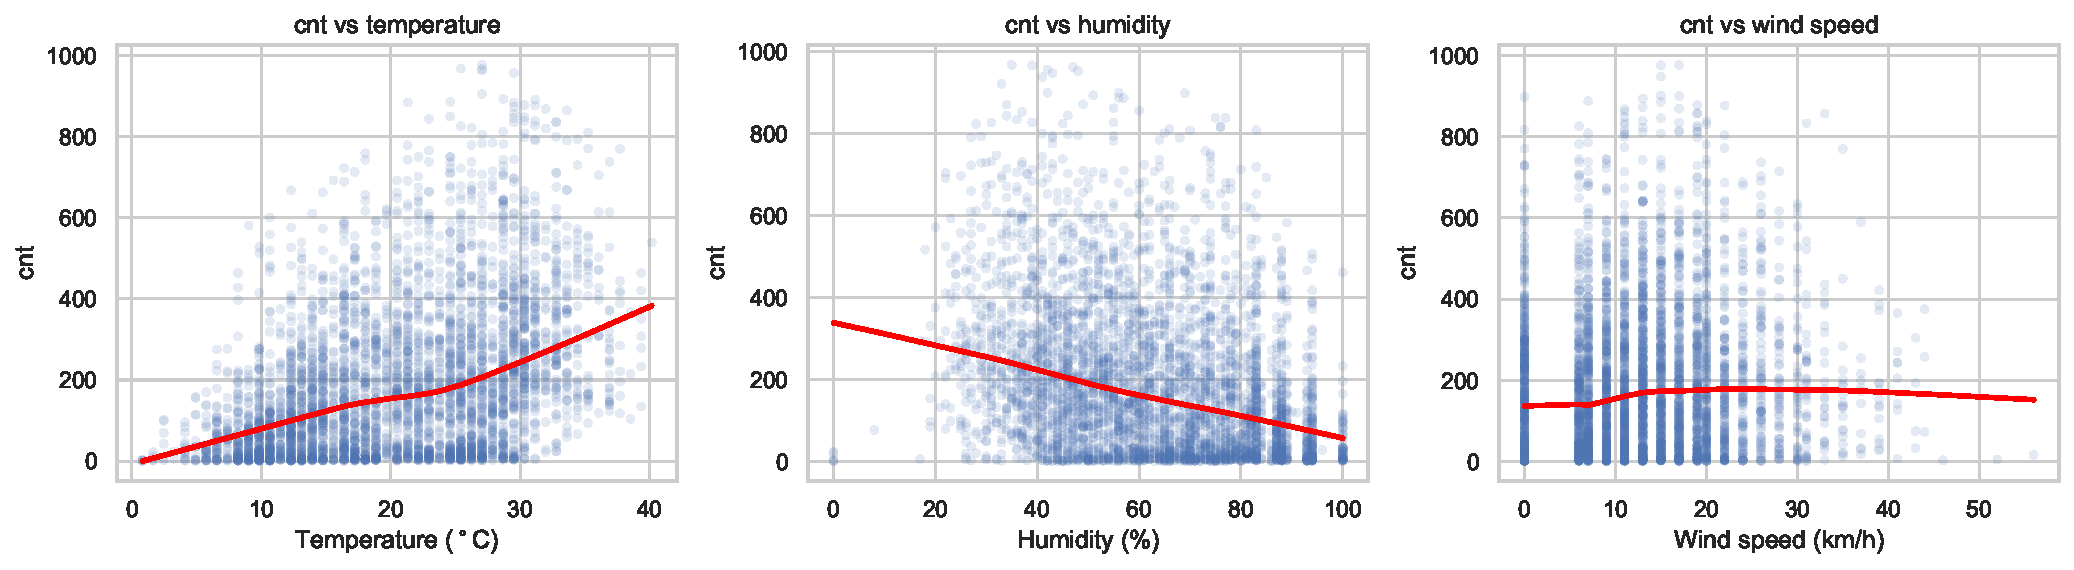
\includegraphics[width=0.98\linewidth]{fig03_weather_scatter.pdf}
\caption{\texttt{cnt} vs.\ the three continuous weather variables,
with lowess smooths in red. Temperature has a clear positive
effect; humidity is clearly negative, especially above 80\%; wind
speed has a mild negative trend with wide spread.}
\label{fig:weather}
\end{figure}

\begin{figure}[H]
\centering
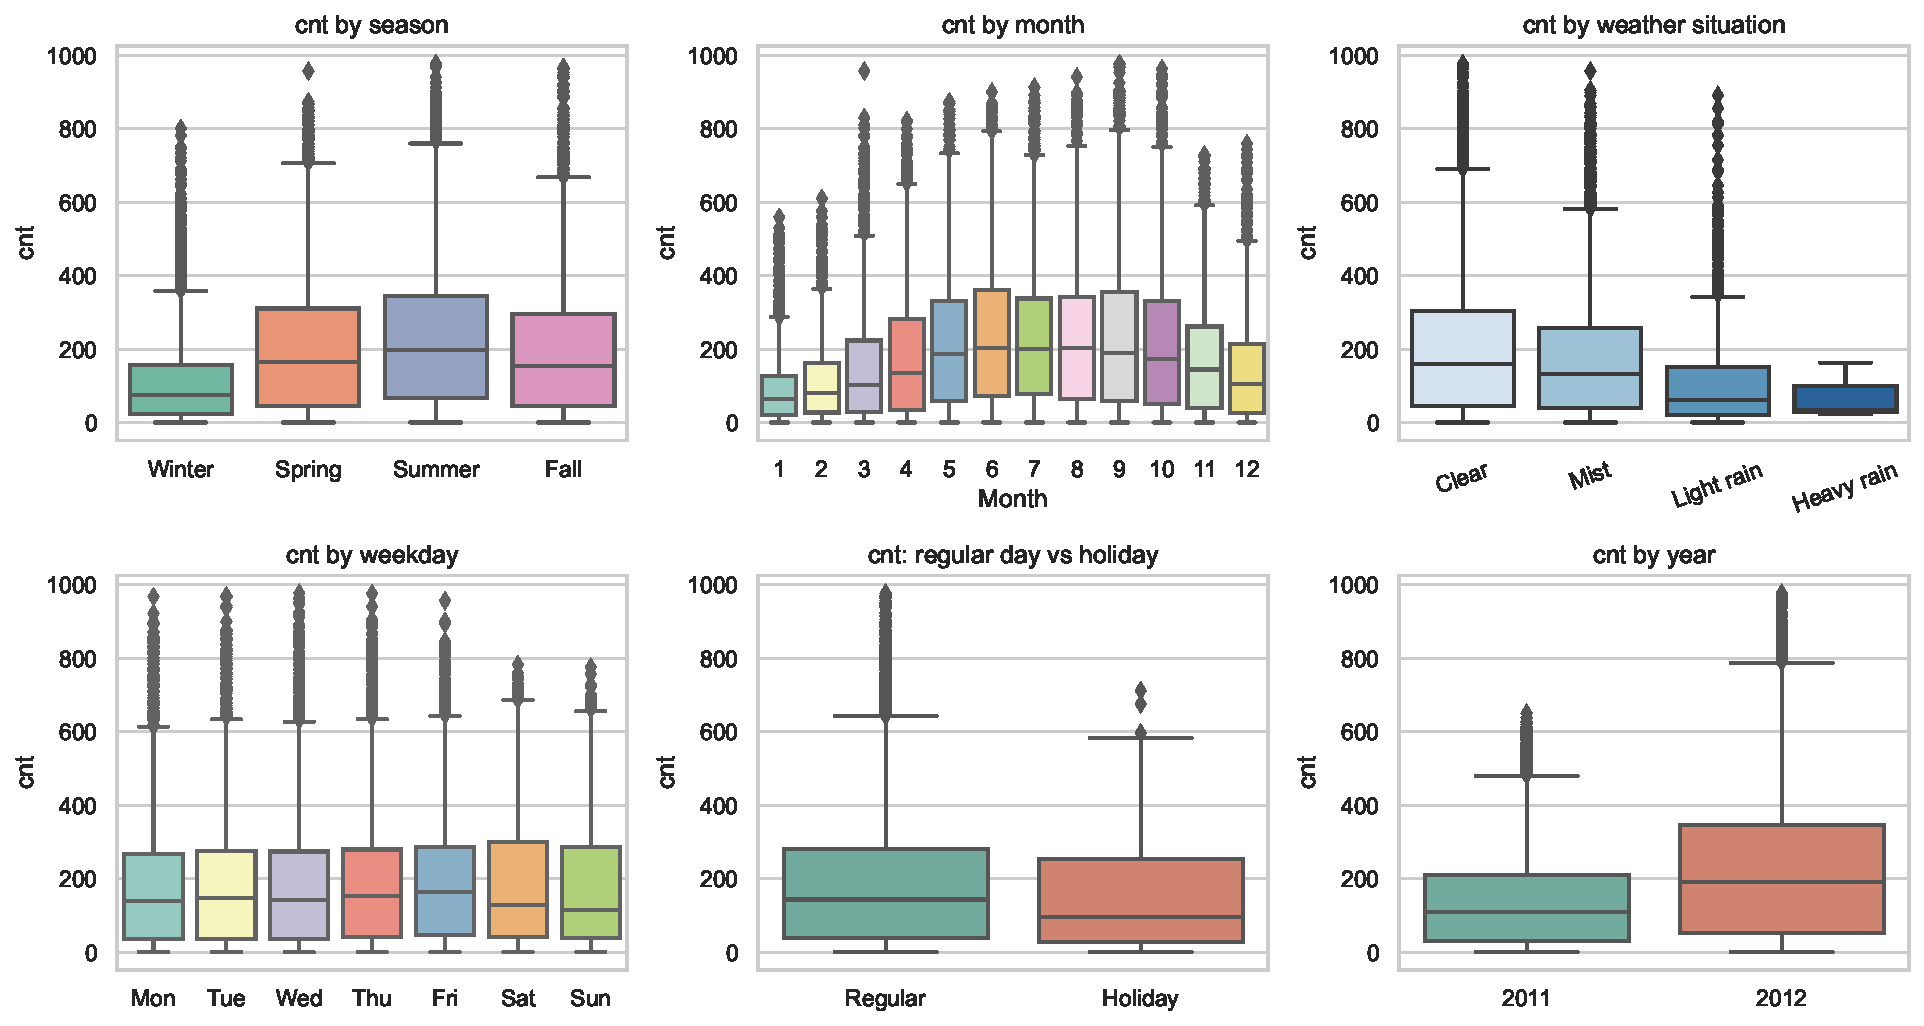
\includegraphics[width=0.95\linewidth]{fig17_categorical_panel.pdf}
\caption{\texttt{cnt} by every remaining categorical / calendar
variable: \texttt{season}, \texttt{mnth}, \texttt{weathersit},
\texttt{weekday}, \texttt{holiday}, \texttt{yr}. Demand has
strong season and month patterns (low winter / Jan--Feb, high
summer / Jul--Sep); \texttt{weathersit} shows a clean monotone
decrease with worsening conditions; \texttt{weekday} marginals are
surprisingly flat (the daytime shape, not the total, is what
differentiates weekdays from weekends); \texttt{holiday} has a
slightly lower median; \texttt{yr} shows the year-over-year growth
from 2011 to 2012 visibly.}\label{fig:catpanel}
\end{figure}

\begin{figure}[H]
\centering
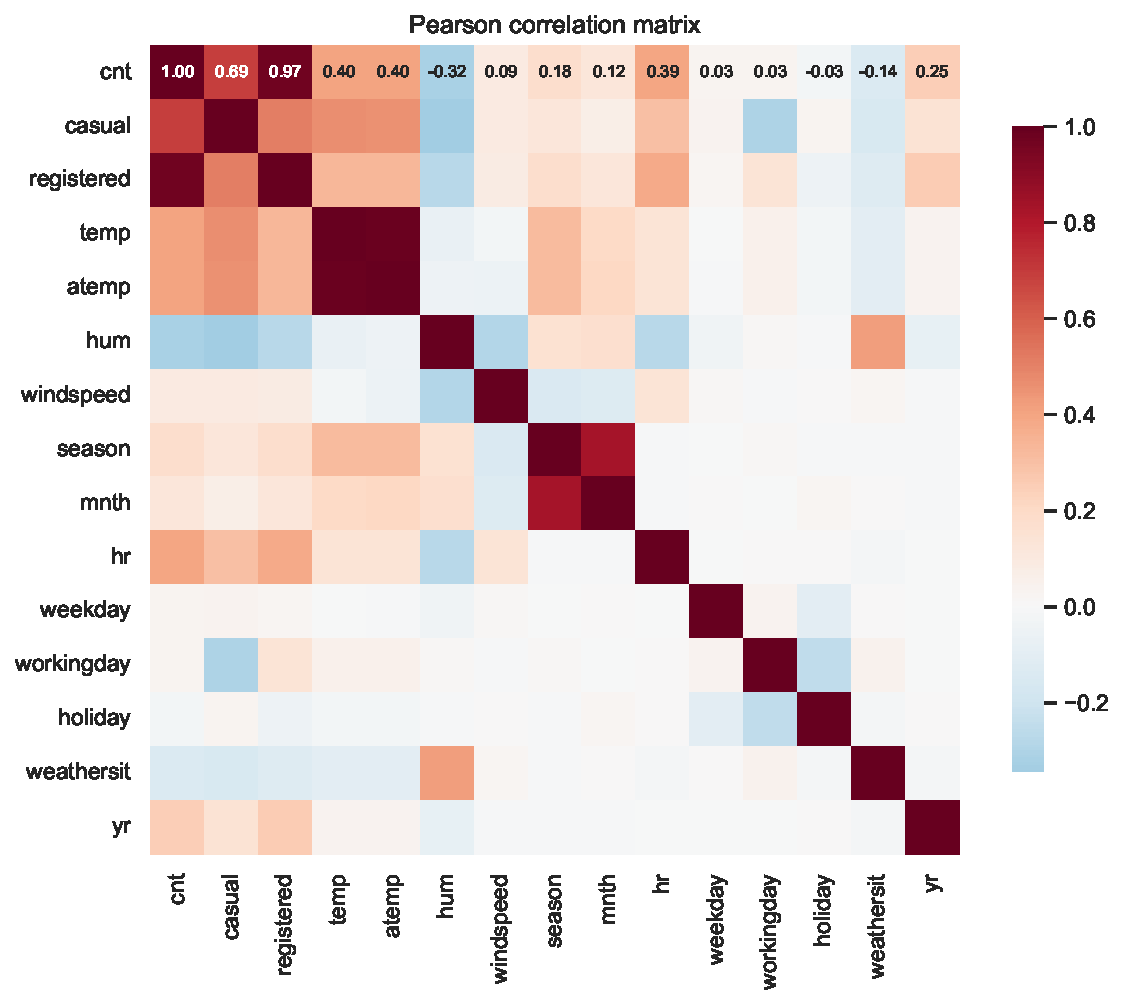
\includegraphics[width=0.82\linewidth]{fig04_correlation_matrix.pdf}
\caption{Pearson correlation matrix. Two redundancies stand out:
\texttt{temp}~$\approx$~\texttt{atemp} ($r=0.99$) and
\texttt{season}~$\approx$~\texttt{mnth} ($r=0.83$). \texttt{cnt}
correlates most strongly with \texttt{temp} ($r\approx 0.40$) and
\texttt{hr} ($r\approx 0.39$); the linear correlation with
\texttt{hr} understates its effect because the relationship is
bimodal.}\label{fig:corr}
\end{figure}

\paragraph{Summary}
The raw target is right-skewed and bimodal-on-log-scale. Demand
peaks twice on working days (08:00, 17:00--18:00) and once midday
on weekends. Temperature is the dominant positive weather driver,
humidity the dominant negative one; wind speed has a mild negative
effect; \texttt{weathersit} decreases demand monotonically with
worsening conditions. Season and month carry the same warm-vs-cold
signal; weekday marginals are nearly flat (the intraday shape,
not the daily total, separates weekdays from weekends); 2012
demand sits visibly above 2011 demand. Two pairs of variables are
essentially redundant
(\texttt{temp}/\texttt{atemp}, \texttt{season}/\texttt{mnth}).

\paragraph{Variables we carry into the unsupervised methods.}
Based on the marginal evidence above, the clustering and factor
analysis use the following eight variables:
\texttt{cnt}, \texttt{temp}, \texttt{hum}, \texttt{windspeed},
\texttt{hr}, \texttt{workingday}, \texttt{season}, and
\texttt{weathersit}.
\texttt{cnt} is included specifically so the clusters organize
themselves around demand level; the other seven are the variables for which the EDA shows a clear marginal relationship with \texttt{cnt}. We drop
\begin{itemize}
\item \texttt{atemp}: redundant with \texttt{temp} ($r=0.99$,
      Fig.~\ref{fig:corr});
\item \texttt{mnth}: redundant with \texttt{season} ($r=0.83$); the
      EDA panel (Fig.~\ref{fig:catpanel}) shows essentially the
      same warm-cold U-shape. We keep the coarser variable for
      clustering and let Lasso choose between them in
      \S\ref{sec:lasso};
\item \texttt{weekday}: marginal effect is nearly flat
      (Fig.~\ref{fig:catpanel}); the only useful binary split
      (weekday vs.\ weekend) is already carried by
      \texttt{workingday};
\item \texttt{holiday}: occurs in only $2.9\%$ of hours --- too rare
      to anchor a cluster on its own;
\item \texttt{instant} and \texttt{dteday}: identifiers, not
      predictors;
\item \texttt{casual} and \texttt{registered}: by construction sum
      to \texttt{cnt}, so leak the target.
\end{itemize}
Factor analysis additionally includes \texttt{yr} because the
2011-to-2012 level shift in Fig.~\ref{fig:catpanel} is a candidate
loading on a ``demand factor''. For clustering we exclude
\texttt{yr}: including it would risk producing a trivial
``2011 cluster vs.\ 2012 cluster'' split that says nothing about
the conditions producing demand.

% =====================================================================
\section{Clustering hourly observations (with \texttt{cnt})}\label{sec:clustering}

We treat each hour as an observation and cluster the $17{,}379$
hours using the feature set
\[
(\texttt{cnt},\ \texttt{temp},\ \texttt{hum},\ \texttt{windspeed},\
 \texttt{hr},\ \texttt{workingday},\ \texttt{season},\
 \texttt{weathersit}),
\]
standardized to mean $0$, variance $1$. Including \texttt{cnt} as a
feature makes the regimes organize themselves around demand
level together with the conditions that produce it.

\paragraph{Choosing $k$.}
Figure~\ref{fig:kmdiag} shows the elbow plot (within-cluster sum of
squares) and the silhouette score for $k = 2,\ldots,8$. The elbow
softens noticeably at $k=4$ and the silhouette has a local maximum
there, so we pick $k=4$. All silhouettes are modest ($\approx 0.17$),
reflecting that the underlying structure is more a continuum of
demand levels than a set of sharply separated balls.

\begin{figure}[H]
\centering
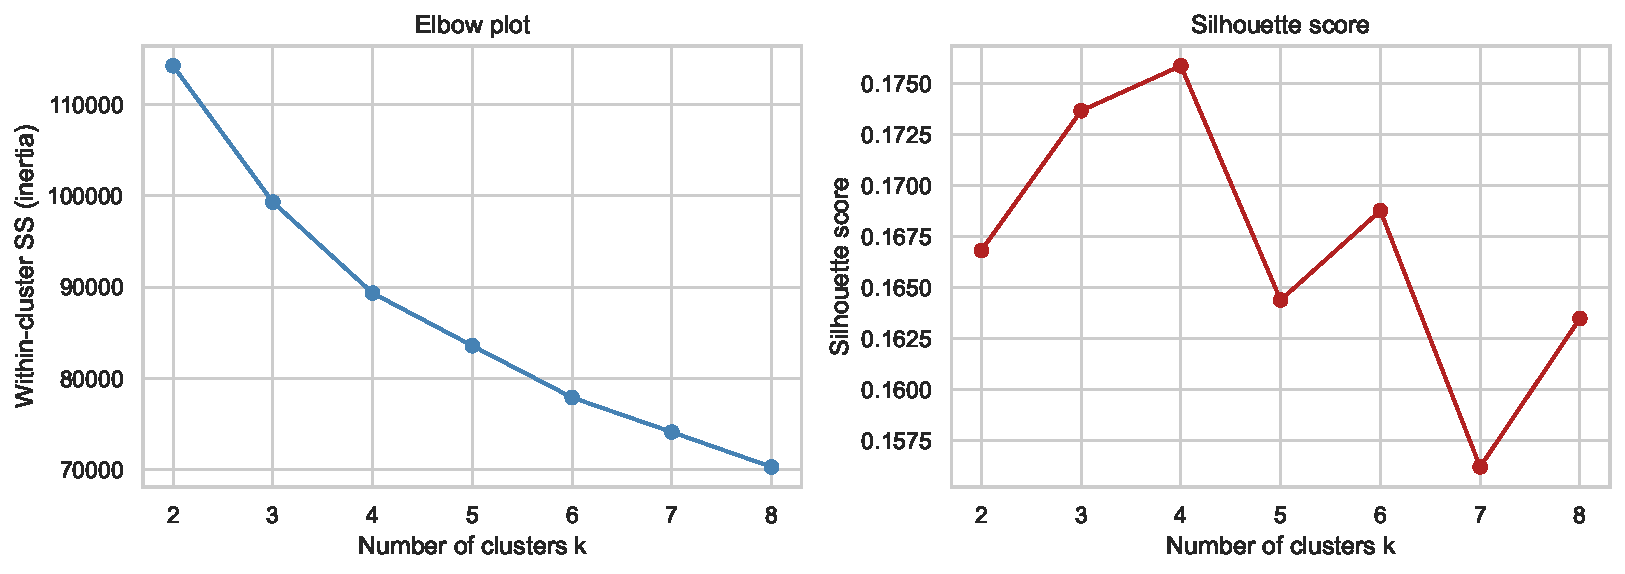
\includegraphics[width=0.95\linewidth]{fig05_kmeans_diagnostics.pdf}
\caption{K-means model selection: elbow plot (left) and silhouette
score (right). $k=4$ is the chosen value.}\label{fig:kmdiag}
\end{figure}

\paragraph{Cluster centroids.}
Figure~\ref{fig:centroids} shows the four cluster centroids on the
standardized features. Red (blue) indicates the cluster sits above
(below) the global mean. Reading the centroid rows together with
the raw-scale means below, we obtain four interpretable regimes:

\begin{center}
\small
\begin{tabular}{c c c c c c l}
\toprule
ID & $n$ & $\overline{\texttt{cnt}}$ & $\overline{\texttt{hr}}$
   & working\% & weathersit & \textbf{label} \\
\midrule
0 & 3,738 & 111 & 11.9 & 66\% & 1.2 & off-peak cool-season hours \\
1 & 6,247 & 347 & 15.8 & 71\% & 1.2 & commuter rush / warm afternoon \\
2 & 4,096 &  57 &  4.1 & 61\% & 1.2 & night hours \\
3 & 3,298 & 144 & 12.2 & 75\% & 2.4 & bad-weather (light rain/mist) \\
\bottomrule
\end{tabular}
\end{center}

\begin{figure}[H]
\centering
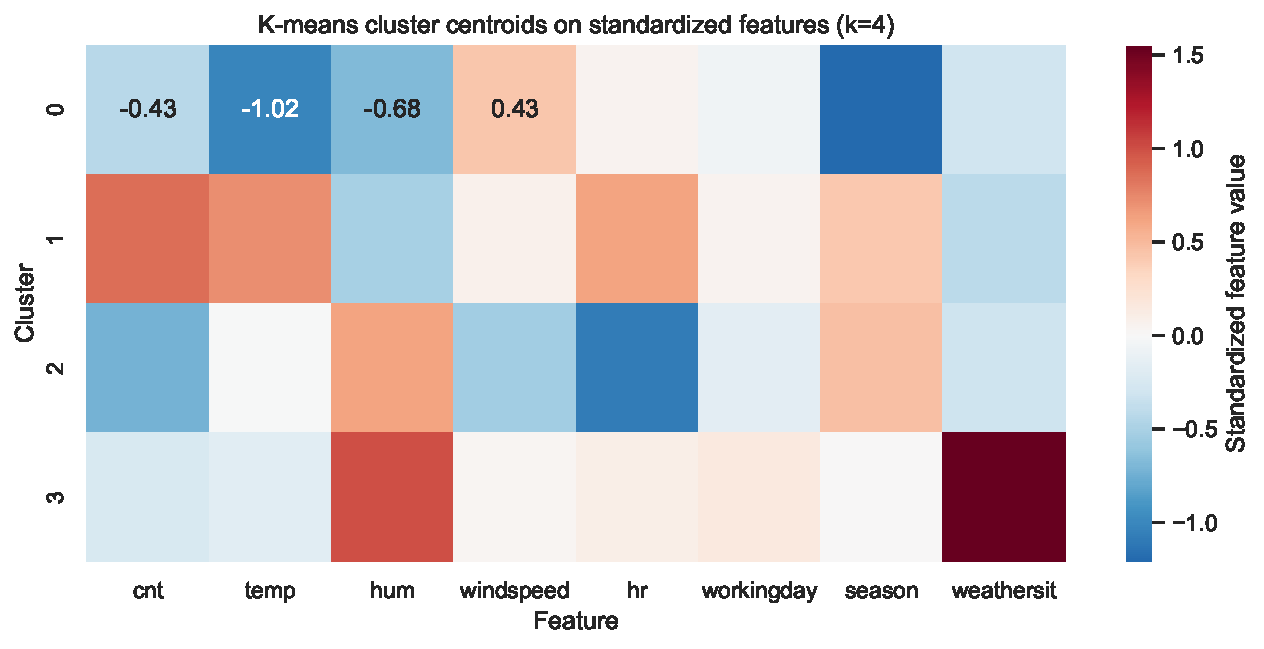
\includegraphics[width=0.95\linewidth]{fig06_cluster_centroids.pdf}
\caption{K-means cluster centroids on the standardized feature
matrix.}\label{fig:centroids}
\end{figure}

\paragraph{Visualizing the clusters in 2D.}
Figure~\ref{fig:pcsc} projects the standardized data onto the first
two principal components. The four K-means clusters form contiguous
regions in the PC1--PC2 plane. The right panel re-colors the same
projection by actual \texttt{cnt}: PC1 is essentially aligned with
demand level, so the clusters are ordered by \texttt{cnt} along PC1
in addition to being separated by hour/weather along PC2.

\begin{figure}[H]
\centering
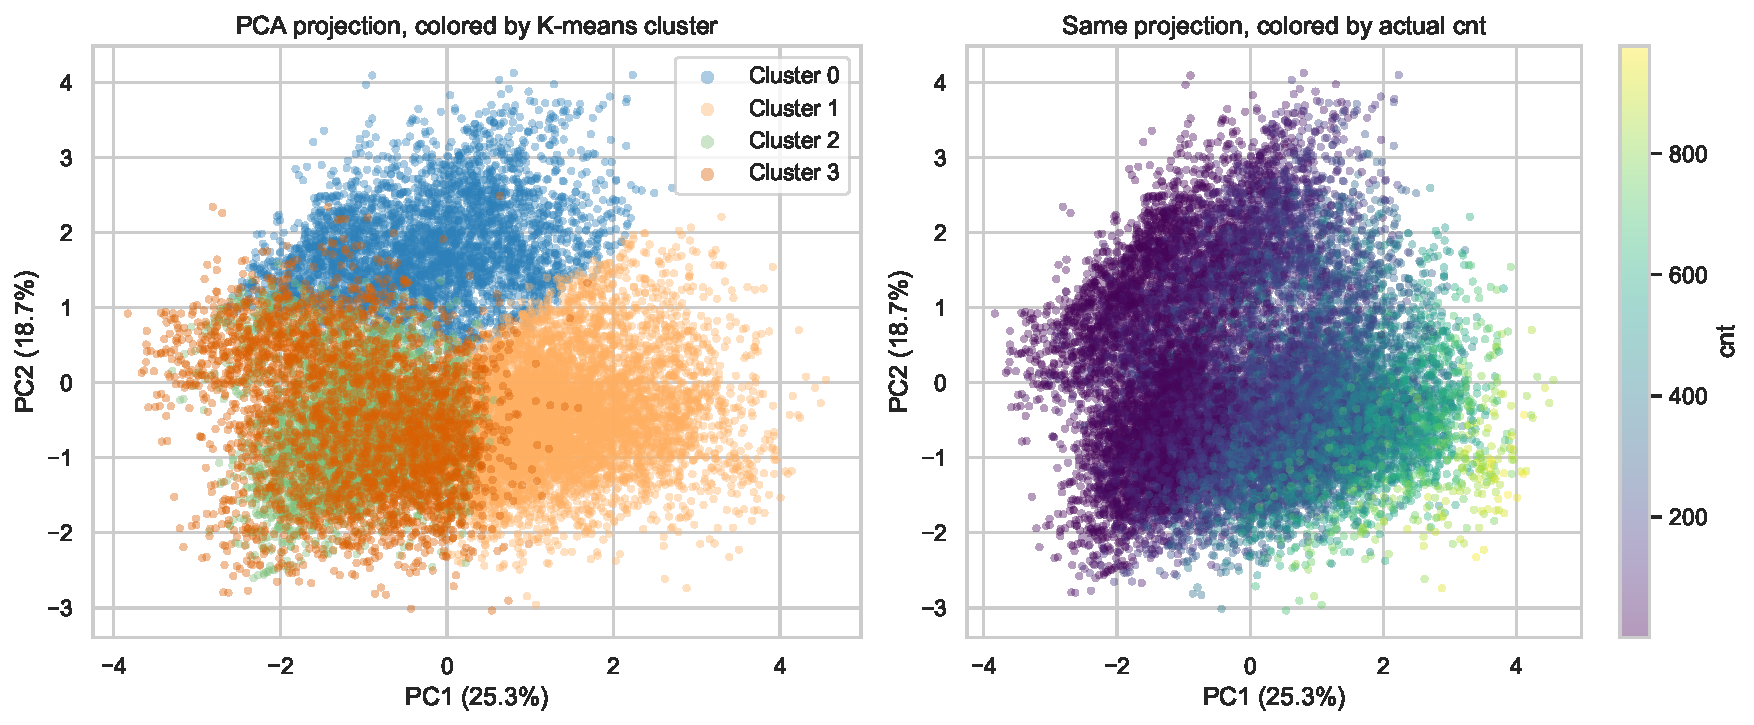
\includegraphics[width=0.95\linewidth]{fig07_cluster_pca_scatter.pdf}
\caption{Left: PC1--PC2 projection of the standardized data,
colored by K-means cluster. Right: same projection, colored by
actual \texttt{cnt}.}\label{fig:pcsc}
\end{figure}

\paragraph{Mean hourly profile per cluster.}
Figure~\ref{fig:cluprof} plots the mean of \texttt{cnt} by hour
within each cluster. The four hourly curves are nicely distinct:
cluster~1 is the high-demand commuter cluster with bimodal peaks at
08:00 and 17:00--18:00; cluster~3 is depressed throughout the day
(bad weather); cluster~0 is the moderate off-peak cool weekday;
cluster~2 is the night cluster, flat and low.

\begin{figure}[H]
\centering
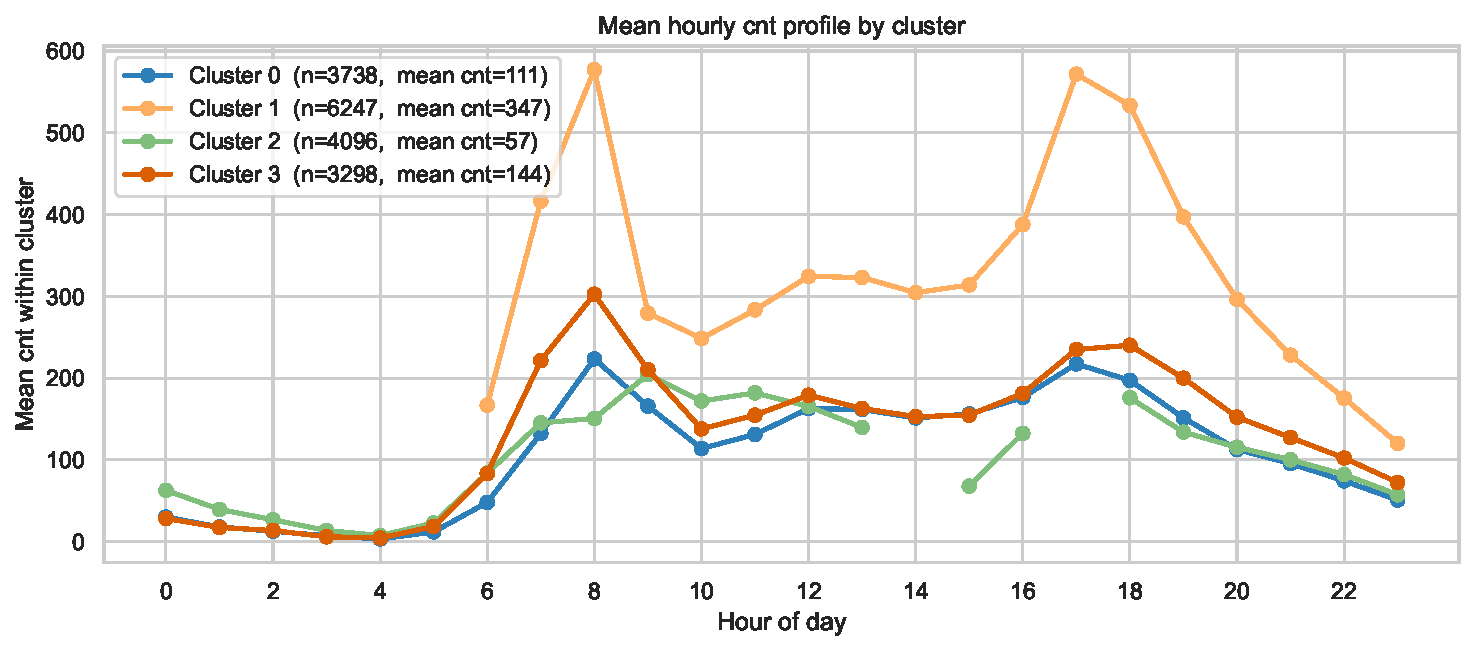
\includegraphics[width=0.92\linewidth]{fig08_cluster_hour_profile.pdf}
\caption{Mean hourly \texttt{cnt} within each K-means
cluster.}\label{fig:cluprof}
\end{figure}

% =====================================================================
\section{Factor analysis of the variable block}\label{sec:fa}

Where clustering grouped observations, factor analysis (FA)
extracts a small number of latent variables (factors) that
explain the covariance among the observed numeric variables. We
apply FA with \textbf{three factors and varimax rotation} to the
same eight variables used in \S\ref{sec:clustering}, augmented with
\texttt{yr} (cf.\ the rationale at the end of \S2: \texttt{yr} is
itself a candidate loading on a demand factor, and FA is not at
risk of producing a degenerate ``year cluster''). We inspect the
resulting loadings to see what each factor represents and how
\texttt{cnt} loads on them.

\begin{figure}[H]
\centering
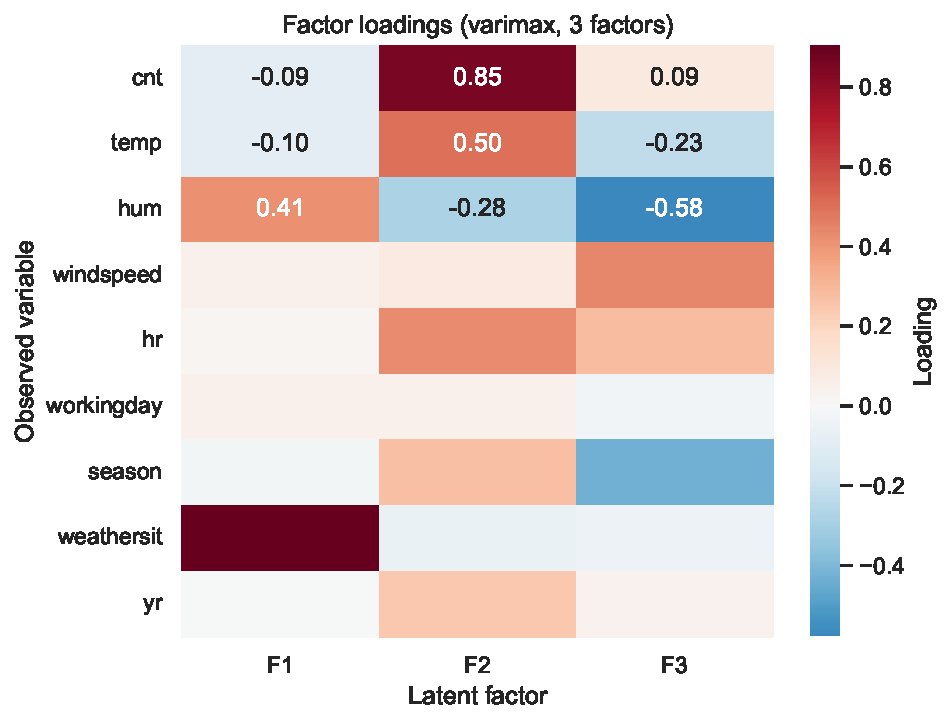
\includegraphics[width=0.6\linewidth]{fig09_fa_loadings.pdf}
\caption{Factor loadings (varimax-rotated, three
factors).}\label{fig:loadings}
\end{figure}

The numeric loadings are:
\begin{center}
\small
\begin{tabular}{l r r r r}
\toprule
variable & F1 & F2 & F3 & communality \\
\midrule
\texttt{cnt}        & $-0.09$ & $+0.85$ & $+0.09$ & 0.74 \\
\texttt{temp}       & $-0.10$ & $+0.50$ & $-0.23$ & 0.31 \\
\texttt{hum}        & $+0.41$ & $-0.28$ & $-0.58$ & 0.59 \\
\texttt{windspeed}  & $+0.05$ & $+0.08$ & $+0.45$ & 0.21 \\
\texttt{hr}         & $+0.02$ & $+0.42$ & $+0.27$ & 0.25 \\
\texttt{workingday} & $+0.05$ & $+0.05$ & $-0.03$ & 0.01 \\
\texttt{season}     & $-0.03$ & $+0.27$ & $-0.43$ & 0.26 \\
\texttt{weathersit} & $+0.90$ & $-0.06$ & $-0.05$ & 0.82 \\
\texttt{yr}         & $+0.00$ & $+0.24$ & $+0.03$ & 0.06 \\
\bottomrule
\end{tabular}
\end{center}

\paragraph{Interpretation of the factors.}

\begin{itemize}
\item \textbf{Factor F1 --- bad-weather factor.}
      Strong positive loading on \texttt{weathersit} ($0.90$) and
      \texttt{hum} ($0.41$). This factor goes up when the weather
      is bad; \texttt{cnt} loads slightly negatively on it.
\item \textbf{Factor F2 --- macro conditions factor.}
      \texttt{cnt} loads heavily on F2 ($0.85$), together with
      positive loadings on \texttt{temp} ($0.50$), \texttt{hr}
      ($0.42$), \texttt{season} ($0.27$), and \texttt{yr} ($0.24$).
      F2 is essentially the macro factor: it bundles together everything that co-varies with high \texttt{cnt}
      --- warm, busy hours, summer/fall, the second year.
\item \textbf{Factor F3 --- residual wind / dry-season contrast.}
      Positive on \texttt{windspeed} ($0.45$) and \texttt{hr}
      ($0.27$); negative on \texttt{hum} ($-0.58$) and
      \texttt{season} ($-0.43$). Roughly: windier, drier, more
      wintery hours.
\end{itemize}

\paragraph{Communalities.}
\texttt{weathersit} ($0.82$), \texttt{cnt} ($0.74$), and
\texttt{hum} ($0.59$) are well summarized by the three factors.
The interesting omission is \texttt{workingday}: its communality is
only $0.01$, meaning the three factors capture essentially none of
its variance. The reason is that \texttt{workingday} affects the
shape of the hourly demand curve (bimodal vs.\ midday hump)
rather than the level of any continuous variable; FA can only
capture linear covariance, and so this important signal is
invisible to it. We will see that Lasso recovers the effect explicitly.

\paragraph{How \texttt{cnt} responds to each factor.}
Figure~\ref{fig:cntfac} bins each factor score into deciles and
plots the mean of \texttt{cnt}. \texttt{cnt} is monotone
increasing in F2 (the demand factor, by construction),
mildly decreasing in F1 (bad-weather), and roughly flat in F3.
The dominant unsupervised story is therefore the two-factor F1/F2
view: bad weather depresses demand; otherwise demand increases with
warmth and time-of-day.

\begin{figure}[H]
\centering
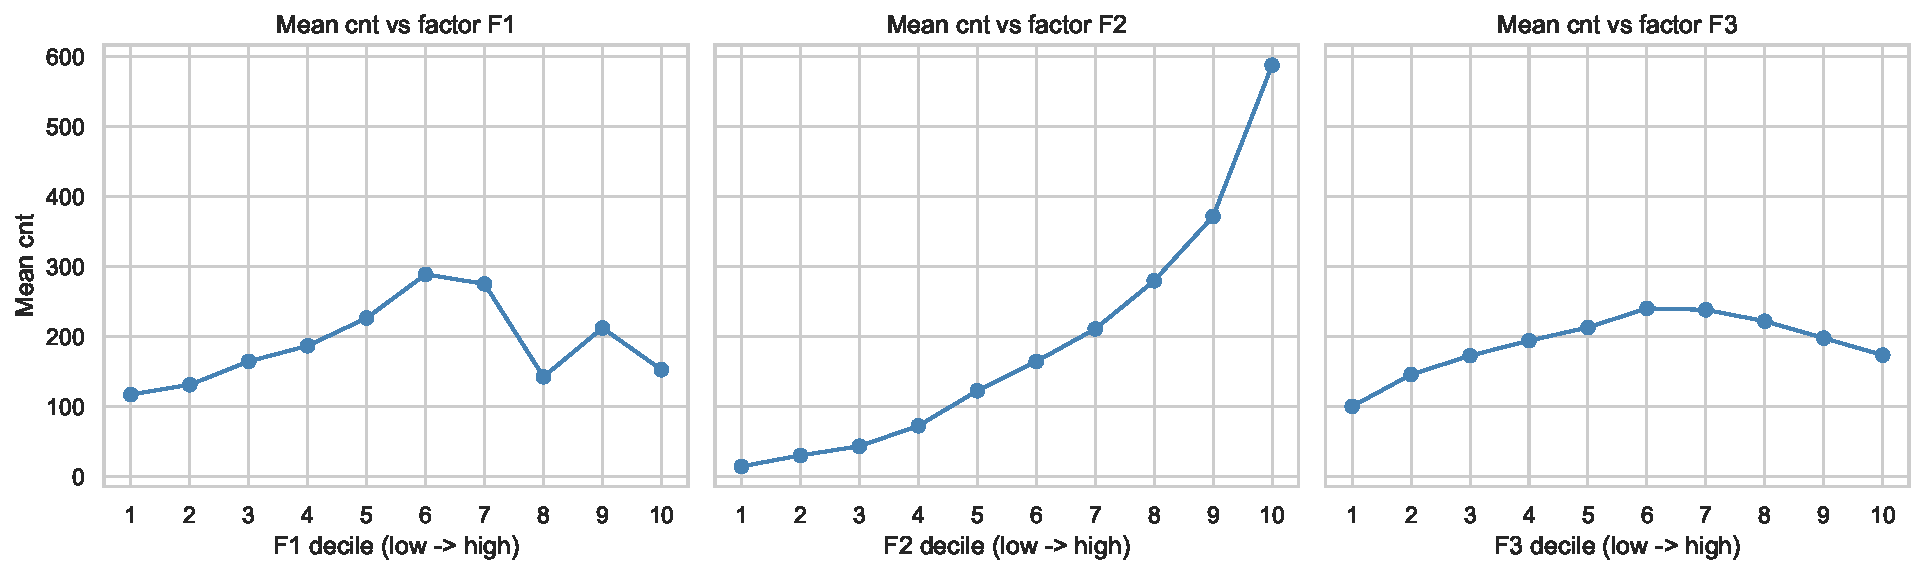
\includegraphics[width=0.95\linewidth]{fig10_fa_cnt_vs_factor.pdf}
\caption{Mean \texttt{cnt} across deciles of each factor
score.}\label{fig:cntfac}
\end{figure}

% =====================================================================
\section{Lasso regression of \texttt{cnt}}\label{sec:lasso}

The third leg of the analysis is supervised. We fit a Lasso to
$y = \log(1+\texttt{cnt})$:
\[
\widehat{\beta}_\lambda
   = \arg\min_\beta\;
     \frac{1}{2n}\|y - X\beta\|_2^2
   + \lambda \|\beta\|_1.
\]
The $\ell_1$ penalty both shrinks coefficients toward zero and
forces some of them exactly to zero, performing automatic
variable selection. The design matrix $X$ contains the continuous
weather predictors \texttt{temp}, \texttt{hum}, \texttt{windspeed},
the year indicator \texttt{yr}, the binary indicators
\texttt{workingday} and \texttt{holiday}, and one-hot encodings of
\texttt{hr} (24 levels $\rightarrow$ 23 dummies), \texttt{weekday}
(7 $\rightarrow$ 6), \texttt{season} (4 $\rightarrow$ 3), and the
merged \texttt{weathersit} (3 $\rightarrow$ 2). All columns are
standardized so coefficient magnitudes are directly comparable;
final design dimension is $17{,}379 \times 40$.

\paragraph{Coefficient paths.}
Figure~\ref{fig:lasso-path} plots each coefficient as a function of
$\log_{10}\lambda$. At large $\lambda$ (left), every coefficient is
zero; as $\lambda$ shrinks, variables enter the model. The ten
variables with the largest unregularized coefficients are
highlighted; the dominant survivors are precisely the
commuter-hour dummies (\texttt{hr\_17}, \texttt{hr\_18},
\texttt{hr\_8}, \texttt{hr\_19}, \texttt{hr\_16}), the late-night
dummies (\texttt{hr\_3}, \texttt{hr\_4}), \texttt{temp},
\texttt{yr}, and \texttt{season\_4}.

\begin{figure}[H]
\centering
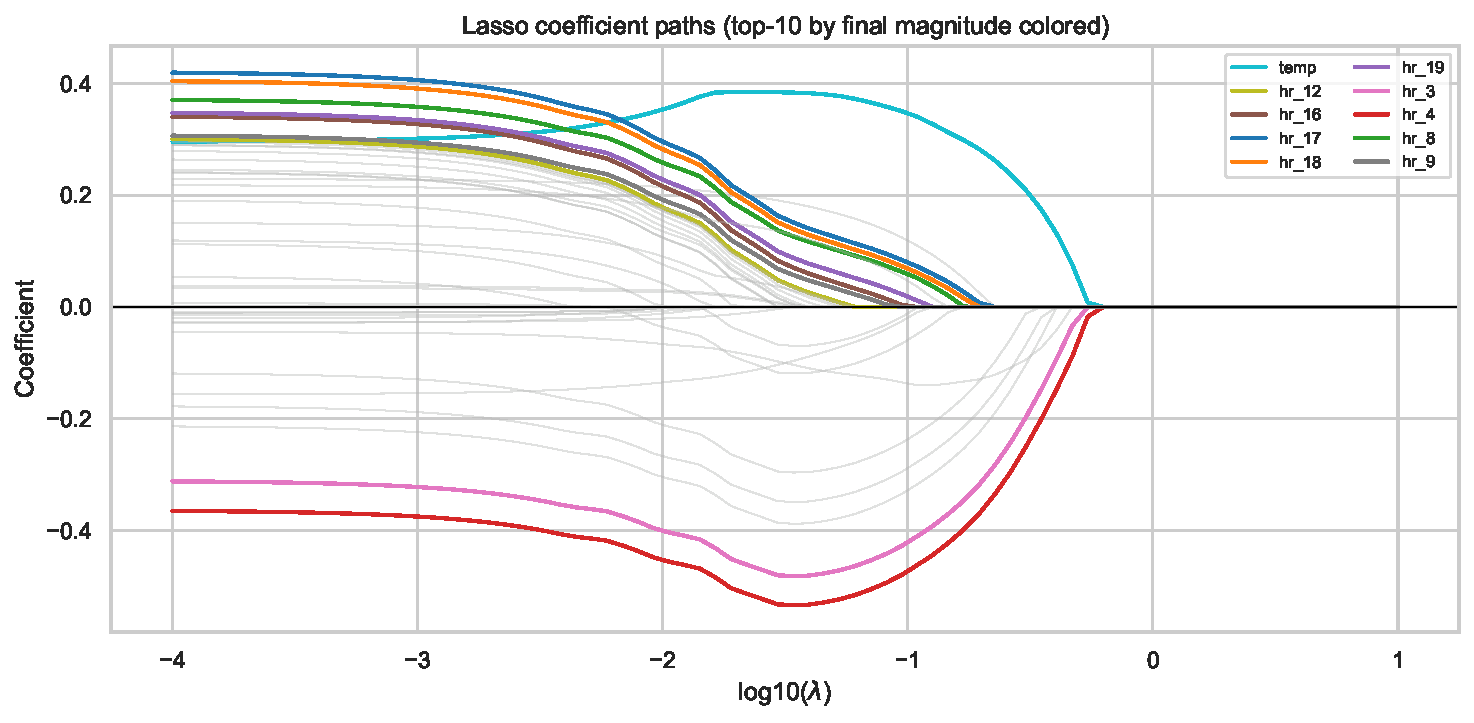
\includegraphics[width=0.95\linewidth]{fig11_lasso_path.pdf}
\caption{Lasso coefficient paths. Each line is the trajectory of
one coefficient as $\lambda$ varies; the ten largest-magnitude
final coefficients are highlighted.}\label{fig:lasso-path}
\end{figure}

\paragraph{Sparsity and fit as $\lambda$ varies.}
Figure~\ref{fig:lasso-r2} shows the number of non-zero coefficients
(left) and the training $R^2$ (right) as a function of
$\log_{10}\lambda$. The number of non-zero coefficients drops from
39 (effectively OLS) at $\lambda \to 0$ to zero at $\lambda > 1$,
with most of the drop concentrated in the range
$\log_{10}\lambda \in [-1.5, +0.5]$.

\begin{figure}[H]
\centering
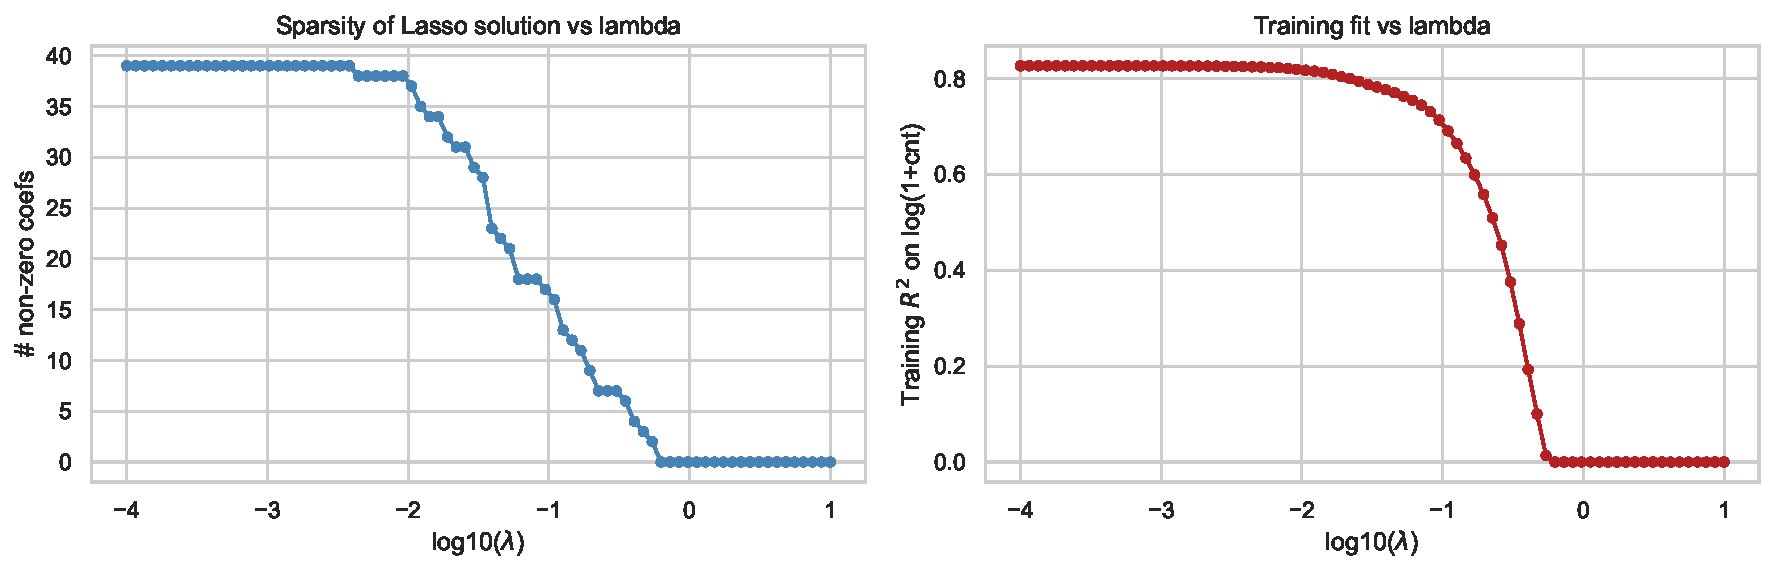
\includegraphics[width=0.95\linewidth]{fig12_lasso_sparsity_and_r2.pdf}
\caption{Lasso sparsity and training fit as a function of
$\lambda$.}\label{fig:lasso-r2}
\end{figure}

\paragraph{On selecting $\lambda$.}
Training $R^2$ is monotone in $\lambda$ (smaller $\lambda$ always
fits the training data better, with $\lambda=0$ recovering OLS), so
it cannot be used to pick $\lambda$. The standard criterion is
out-of-sample prediction error, estimated by
cross-validation: split the data into $K$ folds, for each $\lambda$
train on $K-1$ folds and validate on the held-out one, and
average. The minimizer is conventionally called $\lambda_{\min}$.
A common refinement is the \textbf{1-SE rule}: among all $\lambda$
whose CV-MSE lies within one standard error of $\min$, pick the
largest (most regularized) one. This trades a statistically
insignificant amount of predictive accuracy for a sparser, more
interpretable model.

\paragraph{What CV recommends here.}
Figure~\ref{fig:lassocv} shows the 5-fold CV-MSE curve. It is very
flat in our search range: $\lambda_{\min}$ sits at the lower edge
$10^{-4}$ of our grid, and the 1-SE rule only pushes it to $\lambda_{1\mathrm{SE}} \approx 4.1\times 10^{-3}$. At both of these CV-based choices, all $39$ features remain non-zero.
With $n=17{,}379$ observations and only $40$ features, overfitting is essentially not a concern, so CV legitimately concludes that
``little shrinkage is needed for prediction'' --- but that means CV gives us no help with variable selection.

\begin{figure}[H]
\centering
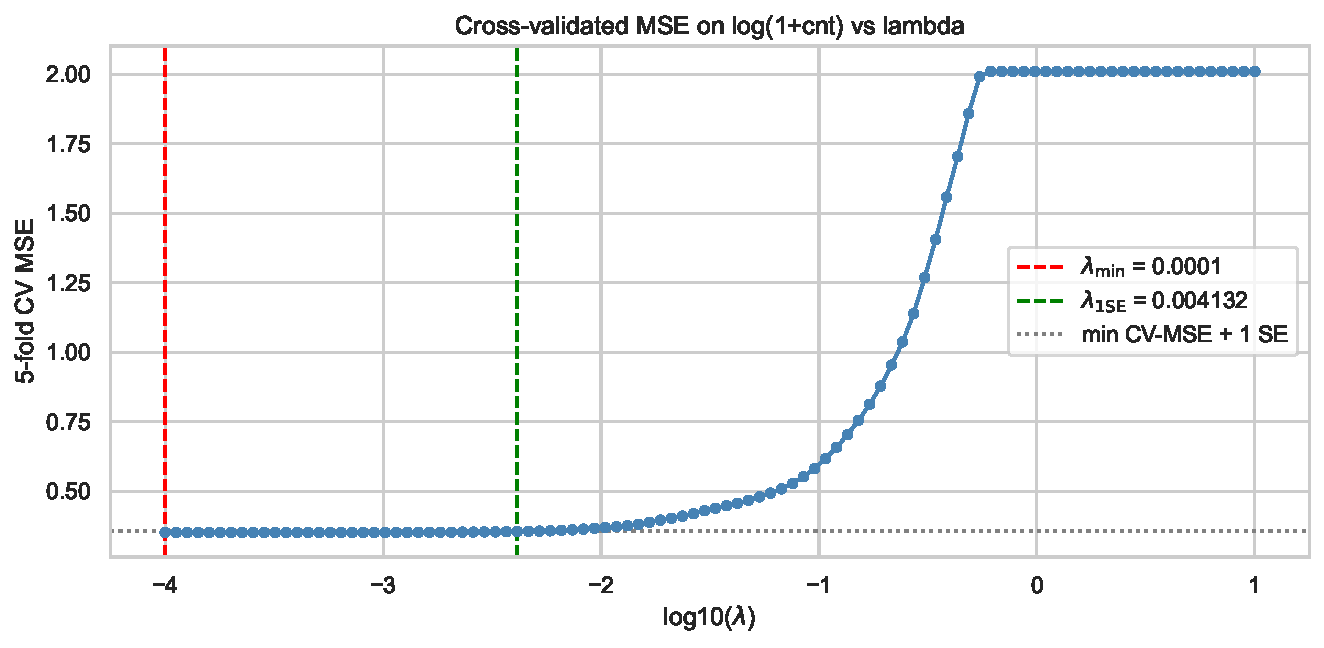
\includegraphics[width=0.85\linewidth]{fig13_lassocv_mse.pdf}
\caption{5-fold CV MSE on $\log(1+\texttt{cnt})$ vs $\lambda$.
Red dashed line: CV-minimum $\lambda$; green dashed line:
1-SE-rule $\lambda$; dotted line: min CV-MSE $+\,1$ SE.}
\label{fig:lassocv}
\end{figure}

\paragraph{Using Lasso as a path tool, not a one-$\lambda$ picker.}
We did not commit to a single ``best'' $\lambda$. For our
$n \gg p$ setting CV recommends essentially no shrinkage (good for
prediction, useless for selection); for variable selection we
instead read the whole Lasso path. Figure~\ref{fig:lasso-multi}
shows the coefficient vector at four representative
sparsity levels (4, 12, 23, 39 features), so the reader can see
how predictive accuracy trades against interpretability:

\begin{center}
\small
\begin{tabular}{r r r p{0.55\linewidth}}
\toprule
$\lambda$ & \# non-zero & $R^2$ & Variables that survive (top by $|\beta|$) \\
\midrule
$0.405$ & 4  & $0.193$ & \texttt{hr\_4, hr\_3, hr\_2, hr\_5}
   --- the four deepest-night hours, all negative \\
$0.146$ & 12 & $0.634$ & adds \texttt{temp}$+$, \texttt{hum}$-$,
   \texttt{yr}$+$, \texttt{hr\_1}$-$, and commuter hours
   \texttt{hr\_17, hr\_18, hr\_8} \\
$0.039$ & 23 & $0.776$ & most \texttt{hr} dummies in,
   \texttt{season\_4}$+$, \texttt{weather3\_3}$-$ \\
$0.004$ & 39 & $0.825$ & all $39$ features ($\approx$ OLS,
   $R^2_{\text{OLS}}=0.826$) \\
\bottomrule
\end{tabular}
\end{center}

The marginal returns are very uneven. Going from $4$ to $12$
variables roughly triples $R^2$; going from $12$ to $23$ adds
$0.15$; going from $23$ to $39$ adds only $0.04$. A reader who
cares about interpretability (knowledge discovery) would
stop somewhere around $\lambda \approx 0.04$ ($\approx 23$
variables, $R^2 \approx 0.78$); a reader who cares about
prediction on this dataset would just use OLS, since
CV does not penalize doing so.

\begin{figure}[H]
\centering
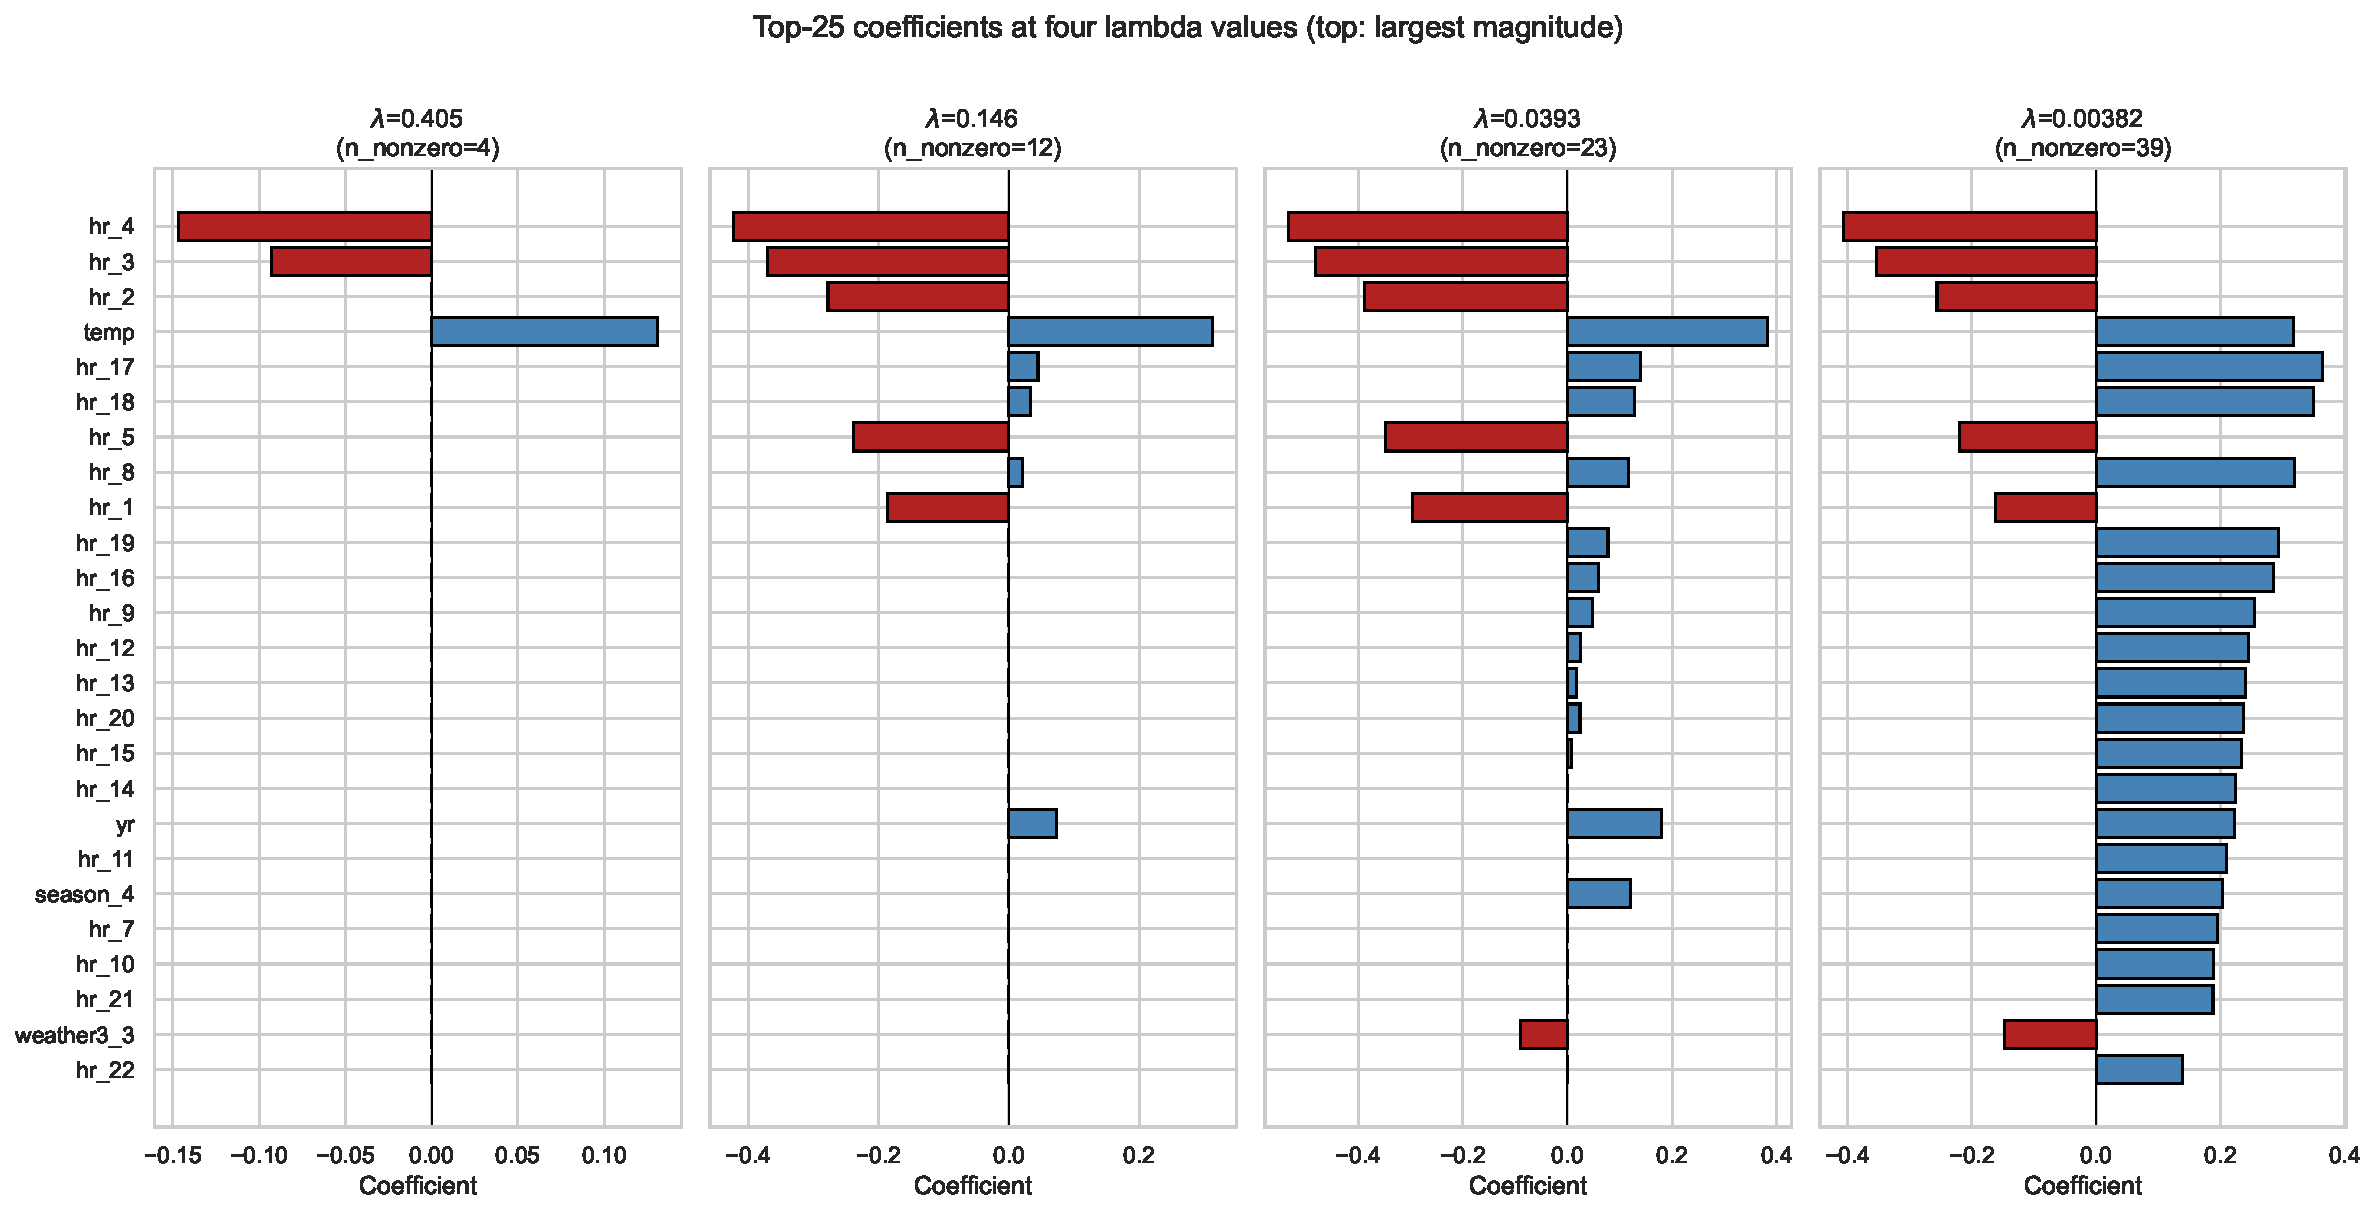
\includegraphics[width=0.95\linewidth]{fig16_lasso_coefs_multiple_lambdas.pdf}
\caption{Top-25 coefficients at four $\lambda$ values, showing how
variables enter the model as $\lambda$ decreases.}
\label{fig:lasso-multi}
\end{figure}

\paragraph{Selected coefficients at $\lambda_{1\mathrm{SE}}$.}
For completeness, Figure~\ref{fig:lasso-coef} shows the (full,
all-$39$-variable) coefficient vector at $\lambda_{1\mathrm{SE}}$.
Even though this $\lambda$ does not drop any variable, the
coefficient pattern itself is informative:

\begin{itemize}
\item Largest positives: \texttt{hr\_17, hr\_18, hr\_8, hr\_19,
      hr\_16} --- commuter peaks.
\item Largest negatives: \texttt{hr\_4, hr\_3, hr\_2, hr\_5, hr\_1}
      --- deep-night hours.
\item \texttt{temp}: large positive coefficient.
\item \texttt{yr}: positive (year-over-year service growth from
      2011 to 2012).
\item \texttt{season\_4} (winter? actually Fall): mild
      positive lift.
\item \texttt{weather3\_3}, \texttt{hum}: negative, as expected.
\item Most \texttt{weekday} dummies and \texttt{workingday} survive
      but with small coefficients --- their information is largely
      carried by the \texttt{hr} dummies.
\end{itemize}

\begin{figure}[H]
\centering
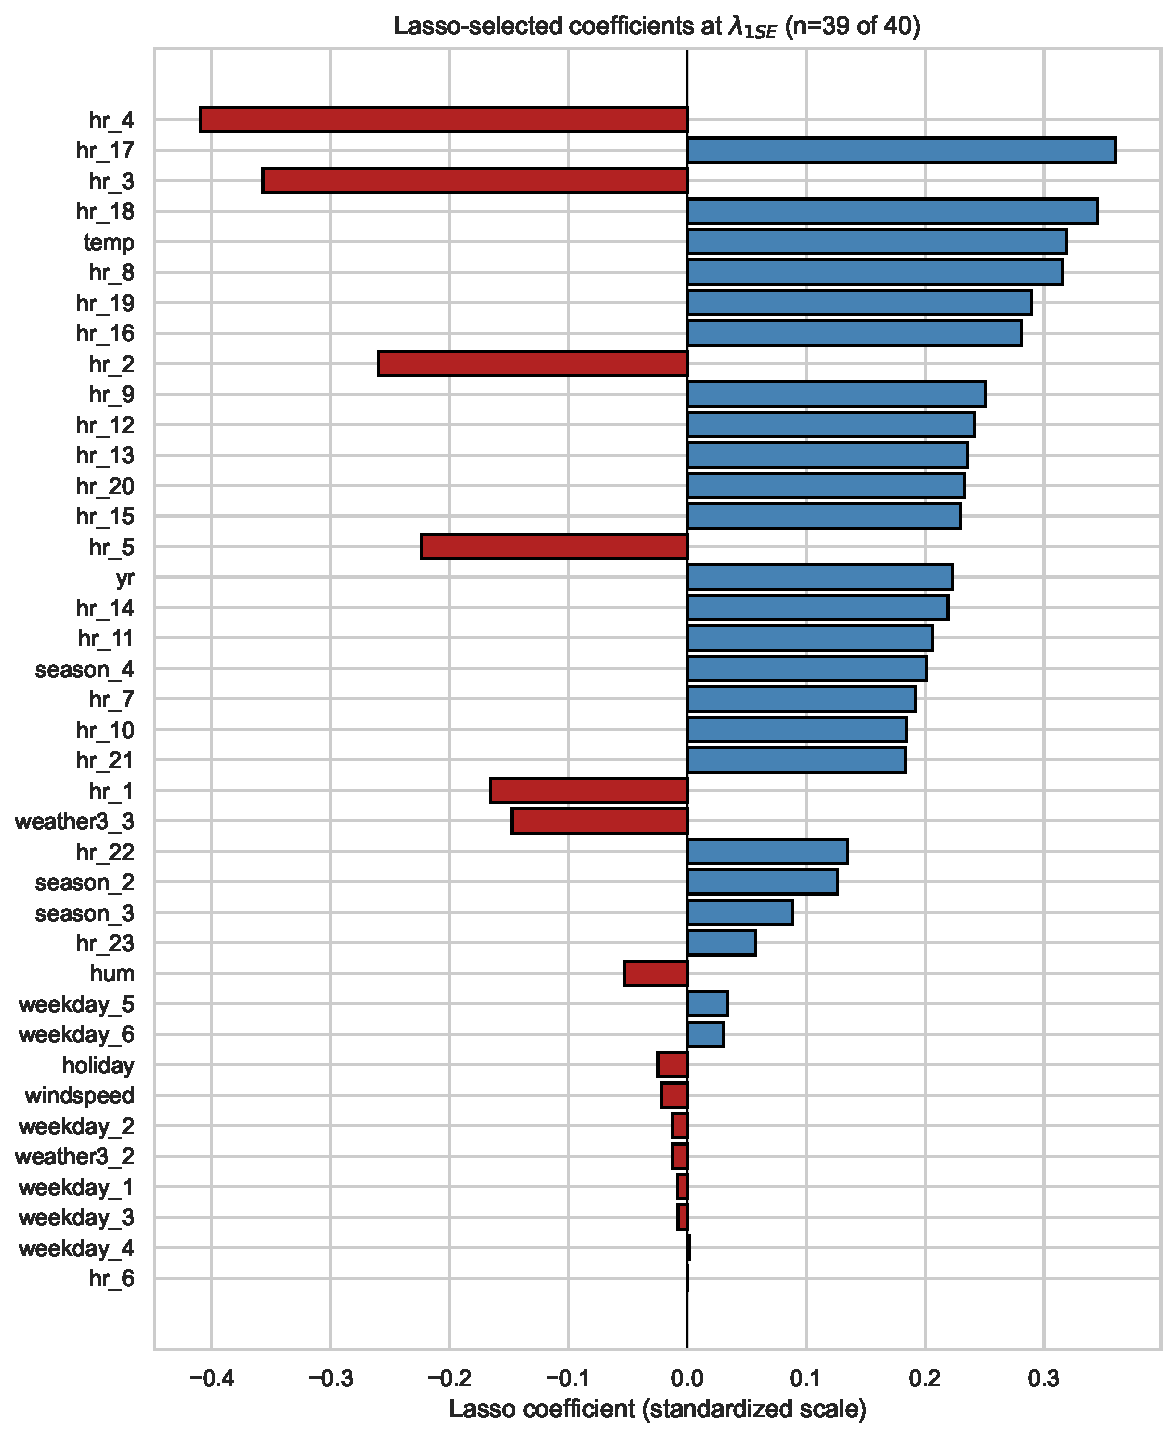
\includegraphics[width=0.85\linewidth]{fig14_lasso_selected_coefs.pdf}
\caption{Coefficients at $\lambda_{1\mathrm{SE}}$. Blue: positive
effect on $\log(1+\texttt{cnt})$; red:
negative.}\label{fig:lasso-coef}
\end{figure}

% =====================================================================
\section{Cross-method comparison and Summaries}\label{sec:compare}

The three methods address the same dataset but answer different
questions. Their conclusions agree on the substantive story but
each highlights a different facet of it.

\subsection*{What each method answers}

\begin{center}
\begin{tabular}{p{0.20\linewidth} p{0.20\linewidth} p{0.50\linewidth}}
\toprule
\textbf{Method} & \textbf{Type} & \textbf{Question it answers} \\
\midrule
K-means & Unsupervised (groups) &
What groups of hours behave similarly, when demand is part of the
similarity criterion? \\
Factor analysis & Unsupervised (latent variables) &
What latent factors explain the covariance among the observed
variables, and how does \texttt{cnt} load on them? \\
Lasso & Supervised (prediction $+$ selection) &
Which variables most strongly predict \texttt{cnt} linearly, and
which can be dropped? \\
\bottomrule
\end{tabular}
\end{center}

\subsection*{What each method reveals}

\textbf{K-means} clusters the $17{,}379$ hours into four
interpretable demand regimes (off-peak, commuter rush, night,
bad-weather) ordered along PC1, which aligns with demand level.
The clusters are descriptive --- they tell us which hours of
the year behave alike.

\textbf{Factor analysis} extracts two dominant latent factors:
F1 = bad-weather (mostly \texttt{weathersit} and \texttt{hum},
with a mild negative on \texttt{cnt}) and F2 = macro factor (with \texttt{cnt}, \texttt{temp}, \texttt{hr},
\texttt{season}, \texttt{yr} all loading positively). A weaker
third wind / dry-winter factor (F3) captures residual
structure. FA misses the \texttt{workingday} effect entirely
(communality 0.01) because that variable affects the shape
of the hourly curve rather than any continuous level.

\textbf{Lasso} is read here as a path rather than a
one-$\lambda$ answer. CV recommends essentially no shrinkage
(the dataset has too much statistical power for shrinkage to help
prediction), so we use Lasso for variable selection instead and
trace which variables enter as $\lambda$ decreases. At an
interpretable sparse level ($\lambda \approx 0.15$, $12$
variables) the model contains the deep-night and commuter-hour
dummies, \texttt{temp}$\,+$, \texttt{hum}$\,-$, and
\texttt{yr}$\,+$ ($R^2 \approx 0.63$). At $\lambda \approx 0.04$
($23$ variables, $R^2 \approx 0.78$) the model adds the remaining
hours, a season dummy, and the bad-weather dummy. Further
reducing $\lambda$ to recover OLS ($39$ features) only adds
$0.04$ to $R^2$.

\subsection*{How the conclusions agree --- and where they differ}

\begin{center}
\begin{tabular}{p{0.30\linewidth} p{0.21\linewidth} p{0.21\linewidth} p{0.20\linewidth}}
\toprule
\textbf{Insight} & \textbf{K-means} & \textbf{FA} & \textbf{Lasso} \\
\midrule
Time-of-day matters
 & implicit (cluster IDs)
 & explicit (F2 loads on \texttt{hr})
 & explicit (most \texttt{hr\_*} dummies) \\
Temperature matters
 & implicit (cluster 1 is warm)
 & explicit (F2 loads on \texttt{temp})
 & explicit ($+$ on \texttt{temp}) \\
Bad weather reduces demand
 & explicit (cluster 3)
 & explicit (F1, $-$ on \texttt{cnt})
 & explicit ($-$ on \texttt{weather3\_3}, \texttt{hum}) \\
Year-over-year growth
 & not surfaced
 & mild loading on F2
 & explicit ($+$ on \texttt{yr}) \\
\texttt{workingday} effect
 & encoded in cluster membership
 & \textbf{missed} (communality 0.01)
 & survives weakly at large $\lambda$ \\
\texttt{temp}/\texttt{atemp} redundancy
 & not addressed
 & absorbed into one factor
 & resolved by dropping \texttt{atemp} \\
\bottomrule
\end{tabular}
\end{center}

The agreement across three different multivariate methods --- each
with a different question and different machinery --- gives strong
confidence that time-of-day, temperature/season, and
weather are the genuine drivers of demand, with a secondary
year-over-year growth term that Lasso surfaces and the
unsupervised methods do not.

A subtler point that the three views collectively expose: factor
analysis misses the workingday effect because that variable
reshapes the hourly profile rather than shifting any continuous
level. Clustering recovers this implicitly via cluster membership
(working-day and weekend hours fall into different clusters
because their \texttt{cnt} levels differ), and Lasso recovers it
via the \texttt{hr\_*} dummies that carry the commuter information.

\subsection*{Summaries for the project}

Two unsupervised methods (K-means clustering with \texttt{cnt}
included as a feature, and varimax-rotated factor analysis)
identify the same two dominant latent dimensions that organize
hourly bike demand: a bad-weather factor and a
demand / favorable-conditions factor that bundles together
hour-of-day, temperature, and season. Lasso, applied with a
different objective (sparse prediction of $\log(1+\texttt{cnt})$),
confirms this by selecting exactly the variables that load on
those two dimensions: hour-of-day dummies (positive at commuter
peaks, negative at night), \texttt{temp}, \texttt{hum}, the year
indicator, and the merged bad-weather dummy. The agreement across
three quite different multivariate methods gives strong confidence
in the substantive picture; the differences --- workingday hidden
in FA, year growth invisible in clustering --- illustrate what
each method does and does not see.

\paragraph{Acknowledgements.}
AI assistance (Claude Code) was used for code boilerplate, plot
styling, and LaTeX typesetting during the exploratory phase,
consistent with the course AI policy. All findings and modeling
decisions are the authors' own.

\end{document}
